% primary responsibility: Phil

\subsection{Blocking}

Figure~\ref{fig:rule_syntax} shows the general syntax for a Snort rule. There are eight types of Snort rules: \texttt{alert}, \texttt{log}, \texttt{pass}, \texttt{active}, \texttt{dynamic}, \texttt{drop}, \texttt{reject}, and \texttt{sdrop}. Each type is described below:

\begin{itemize}
    \item \texttt{alert}.
        \texttt{alert} is the most commonly used type of rule. It sends an
        alert to who ever is running the Snort server \emph{and} logs the
        packet(s) for later inspection.

    \item \texttt{log}.
        \texttt{log} logs the packet that triggered the rule, but does not send
        an alert. This can be used for a rule that is not critical but the
        network administrator wants to be able to look at it later.

    \item \texttt{pass}.
        \texttt{pass} does not do anything with the packet. The packet is
        ignored and allowed to proceed to its destination. This is a way of
        turning off a rule that is not necessary.

    \item \texttt{active}.  The is the same as \texttt{alert} except that after
        sending an alert, a dynamic rule is turned on.

    \item \texttt{dynamic}.  A \texttt{dynamic} rule will do nothing until
        activated by an \texttt{active} rule. Once it has been activated, it
        acts as a \texttt{log} rule.

    \item \texttt{drop}.  \texttt{drop} blocks the packet and logs it. This
        only works if Snort is in inline mode.

    \item \texttt{reject}.
        \texttt{reject} blocks the packet (if in inline mode), logs it, and
        sends a TCP reset message (for a TCP connection) or a ICMP port
        unreachable message (for UDP connection) to both ends of the connect.

    \item \texttt{sdrop}.
        Same as \texttt{drop} except that the packet is not logged.
\end{itemize}

For the purposes of blocking websites, we are interested in \texttt{drop},
\texttt{reject}, and \texttt{sdrop}. We want to be record when a website is
being blocked (we want the packet logged), so \texttt{sdrop} does not fit our
needs. For \texttt{drop} to work correctly, Snort needs to configured in inline
mode. Inline mode is when the Snort server is inline with Internet traffic. For
example, the Snort server would be between the local network and the Internet
connection. All data is inspected by the Snort server and either blocked or
passed through. As our design section describes, this configuration has
important implications. This means that if the Snort server fails then the
Internet connection will be lost. This also means that the Snort server could
potentially act as a bottle neck, slowing down traffic. Because of these
reasons, we decided that putting Snort inline in the network did not fit our
needs. This means that \texttt{block} is not a valid action.

The last rule action is reject. Since we are concerned about blocking HTTP
requests, we concern ourselves with only the TCP functionality of reject and
ignore the UDP functionality. Reject uses a well studied TCP attack called TCP
Reset attack~\cite{watson2004slipping}.

\begin{figure}[!t]
    \centering
    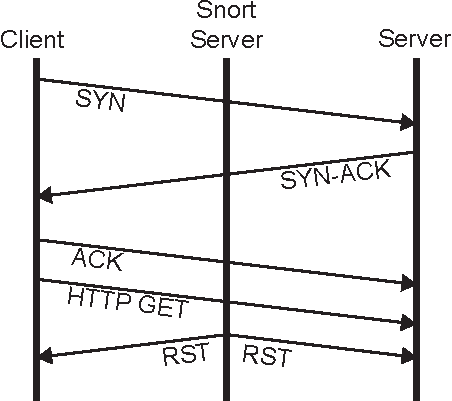
\includegraphics[width=.8\columnwidth]{figures/tcp_reset}
    \caption{The flow of how a TCP RST attack works in our system. When the
    Snort server detects a HTTP GET request, the Snort server sends a TCP RST
    packet to both ends of the connection (Client and Server).}
    \label{fig:tcp_reset}
\end{figure}

For a TCP Reset attack to work, there must be a man in the middle. It monitors
the TCP connections that are being made between the network and the Internet.
When the man in the middle wants to stop a connection, it sends a TCP RST packet
to both ends of the connections. Both ends of the connection think that the
packet came from the other end so it honors the RST packet. For this to work,
the man in the middle must know the sequence number and ACK number of the TCP
stream. This can easily be found by looking at the header of TCP packets. Once
both ends of the connect receive the TCP RST packet, they stop sending data and
close the connection. Figure~\ref{fig:tcp_reset} shows a packet flow of a TCP
reset attack.

\begin{figure*}[!hbtp]
    \centering
    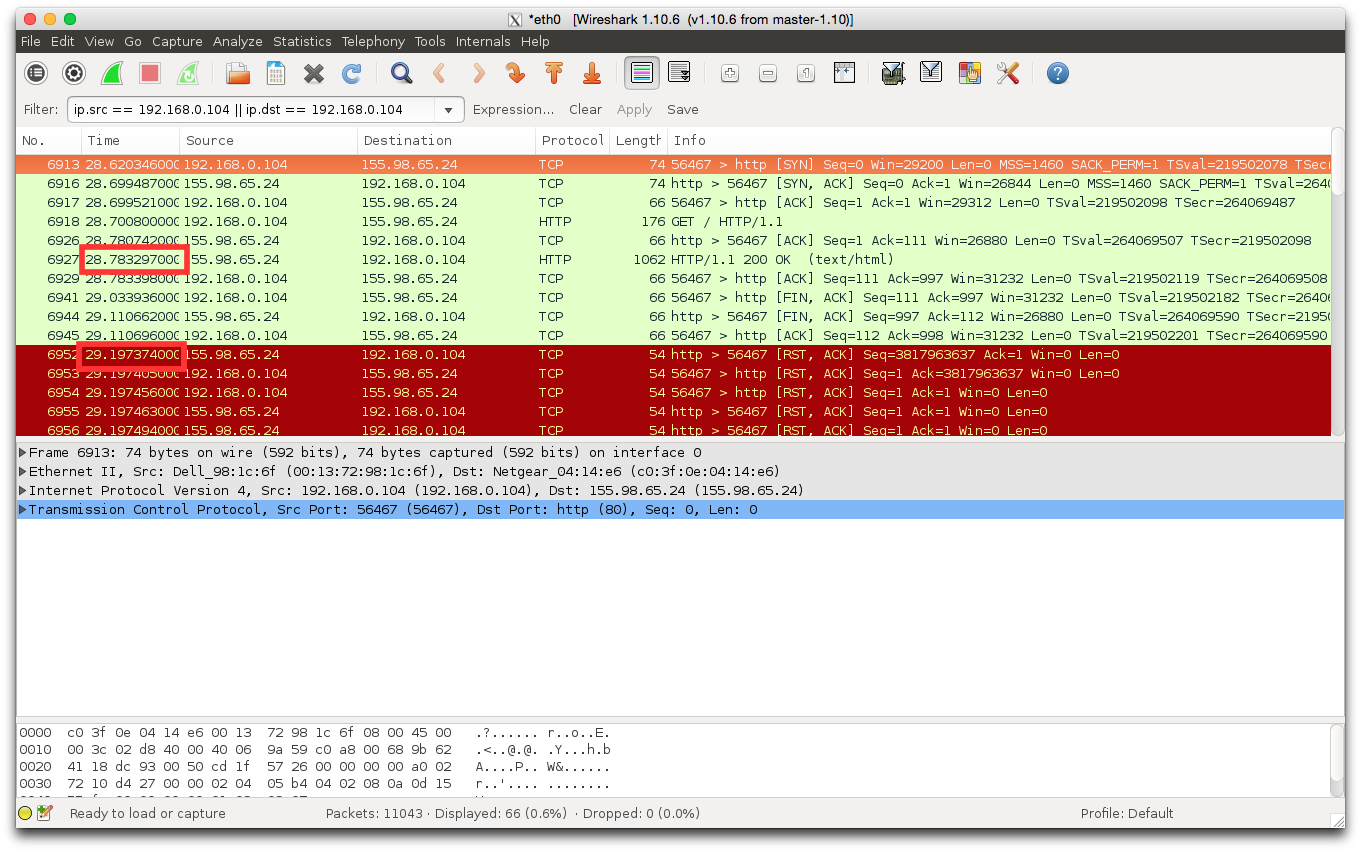
\includegraphics[width=2\columnwidth]{figures/snort_slow}
    \caption{A screenshot of a Wireshark trace. In this trace, the Snort
    server is .41 seconds too late in sending TCP RST packets.}
    \label{fig:snort_slow}
\end{figure*}

In the case of our system, the Snort server is the man in the middle. When a
reject rule is triggered, the Snort server sends a TCP RST packet to each end
of the connection.

Snort's reject rule works in theory, but in practice it has some problems.
%
An inherent issue with not having our Snort server inline but instead having
it rejecting connections is that there could be conditions such that a TCP
connection could finish transmitting all of its data before the Snort server
has time to respond.
%
This is exactly what happens under certain conditions.
%
Figure~\ref{fig:snort_slow} shows a screenshot of a Wireshark trace.
%
In it, the TCP connection is established, data is sent, and then the Snort
server sends its TCP RST packets.
%
The time between when the data is received by the client and when the Snort
server sends a TCP RST packet is .41 seconds.

To really understand the problem with Snort being slow, we ran Snort in many
different environments to make sure it wasn't a platform or topology specific
problem. We ran the server on a MacBook Pro running OS X 10.10, a home network
server running Ubuntu 14.04, and on an Emulab~\cite{emulab} node running Ubuntu
14.04. In the first two environments, the same problems occurred -- Snort would
not react fast enough to block all TCP traffic. In the third environment, we
couldn't test a web server on the Internet (because of how Emulab is set up),
but Snort was able to block a web server that was part of the Emulab
experiment.

After some experimentation, there seems to be two factors that play a role in
if the Snort server is able to reject a TCP connection or not. The first is the
latency involved in making the request. If the request is being made to a
server that is near by geographically, the Snort server has a harder time
blocking it because the connection is so fast. The second factor is how big the
web page that is being downloaded. In our tests, we found that Snort was unable
to block web pages that could be contained inside one TCP packet. However, if
web page was large enough that there needed to be a few packets to send the
data, then Snort could block it most of the time. This was also true with large
images as well.

To try to minimize this problem, we tried reducing the functionality of Snort.
Snort is a IDS and has a lot more functionality that we don't need to block
websites. By reducing what Snort is loading in its configuration, we can speed
up the response time of the TCP RST packets. This helped to reduce the problem,
but it did not fix it. In the future, we plan on looking at the source code of
Snort and pulling out only the necessary parts to block websites.


% Prevent the subsection heading from appearing with a figure between it and
% its first paragraph.
\vspace{20mm}
\subsection{Creating the Whitelist}

\begin{figure}[!tb]
    \centering
    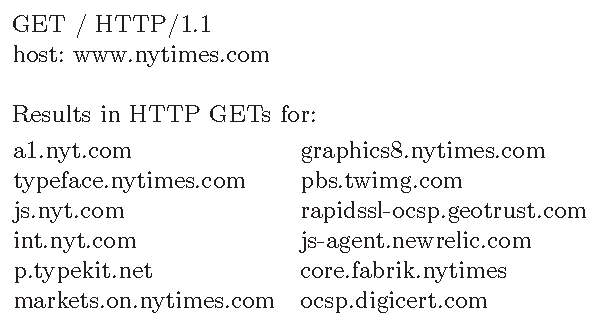
\includegraphics[width=\columnwidth]{figures/http_get}
    \caption{One HTTP GET request results in many more HTTP GET requests. Some
    of these requests are to different domains.}
    \label{fig:http_get}
\end{figure}

Part of being able to block websites adequately is being able to produce a
good list of URLs that should not be blocked (a whitelist). This is harder than
it first sounds. This is in part due to the complexities of the Internet.
Typically, when a web page is visited, resources from many different locations
are loaded. An example of this is shown in Figure~\ref{fig:http_get}. This
makes creating a realistic whitelist much more difficult. For example, a URL
might be added to the whitelist, but for all of the websites important
resources (images, fonts, etc.), other URLs need to be added to the whitelist
as well. It becomes a lot harder as a parent to know what should be added to
the whitelist.

To understand what a whitelist might look like for a typical family, one of the
authors allowed for their families Internet traffic to be logged. This was done
by using \texttt{tshark}~\cite{tshark} (a terminal version of Wireshark) to
monitor Internet traffic and output the host name of a HTTP GET request to a
file. This gave us insight into what kind of considerations need to be made
when building an accurate whitelist.

